% Capítulo 2: Marco teórico.

Este capítulo reúne los fundamentos necesarios para seguir el resto de
la memoria. Se parte de la selección de características y de su
formulación combinatoria como problema de optimización, y se introducen
después la computación cuántica adiabática y el bloqueo de Rydberg en
plataformas de átomos neutros, que sostienen el método cuántico
evaluado. Una sección adicional describe las herramientas de validación
estadística empleadas para distinguir resultados sólidos de relaciones
espurias. El capítulo termina relacionando estos fundamentos con las
decisiones concretas del trabajo.

\section{Selección de características}
\label{sec:mt-fs}

En aprendizaje automático supervisado, la selección de características
consiste en identificar el subconjunto de variables predictoras que
conserva la capacidad predictiva del problema reduciendo
dimensionalidad, redundancia y coste computacional~\cite{guyon2003}.
Sus beneficios habituales son tres: modelos más simples y más
interpretables, menor riesgo de sobreajuste cuando el número de
variables es alto en relación con el de muestras, y menor coste de
entrenamiento e inferencia. En espacios de alta dimensionalidad estos
beneficios dejan de ser una optimización y pasan a condicionar la
validez de las conclusiones, porque una parte de la señal aparente
puede deberse al azar de los contrastes múltiples.

Los métodos de selección se agrupan habitualmente en tres
familias~\cite{guyon2003}. Los métodos \emph{filter} puntúan cada
variable (o subconjunto) con un criterio estadístico independiente del
modelo, como los contrastes univariantes o la información mutua. Los
métodos \emph{wrapper} evalúan subconjuntos entrenando repetidamente un
modelo y midiendo su rendimiento. Los métodos \emph{embedded} obtienen la
selección como subproducto del propio entrenamiento, como ocurre con la
regularización $\ell_1$ o con las importancias de los modelos de
conjunto. Dentro de los filtros conviene distinguir además los criterios
\emph{supervisados}, que miran el target (contrastes univariantes,
información mutua), de los \emph{no supervisados}, que no lo usan. La
varianza es el ejemplo más simple de filtro no supervisado: puntúa cada
variable por su dispersión, sin mirar la etiqueta. En este trabajo se
incluye precisamente con ese papel, como control sin target frente al
resto de selectores supervisados~\cite{solorio2020}.

Una pieza central de muchos criterios de selección es la información
mutua~\cite{cover2006}. Para una variable $X$ y un target $Y$, la
información mutua $I(X;Y)$ mide la dependencia estadística entre
ambas, lineal o no lineal, y se anula únicamente cuando son
independientes:
\begin{equation}
  \label{eq:mi}
  I(X;Y) = \sum_{x \in X} \sum_{y \in Y} p(x,y)\,
  \log\frac{p(x,y)}{p(x)\,p(y)},
\end{equation}
donde $p(x,y)$ es la distribución conjunta de $X$ e $Y$, y $p(x)$ y
$p(y)$ sus distribuciones marginales. Esta generalidad la hace adecuada
tanto para medir la
\emph{relevancia} de una variable respecto al target como la
\emph{redundancia} entre pares de variables. Seleccionar solo por
relevancia tiende a producir subconjuntos redundantes, donde varias
variables aportan información solapada; el criterio mRMR
(\textit{minimum Redundancy Maximum Relevance})~\cite{peng2005}
formaliza el compromiso entre ambas cantidades y lo resuelve de forma
voraz, añadiendo en cada paso la variable que maximiza la relevancia
penalizada por la redundancia con las ya elegidas.

\section{Formulación combinatoria del problema}
\label{sec:mt-qubo}

Elegir el mejor subconjunto de $k$ variables entre $p$ candidatas es
un problema combinatorio: el número de subconjuntos crece
exponencialmente y la búsqueda exacta resulta intratable salvo en
espacios muy pequeños. Esta es la razón de que los métodos clásicos
recurran a heurísticas voraces o a criterios univariantes que no
garantizan el óptimo global.

El compromiso relevancia--redundancia admite una formulación exacta
como problema de optimización binaria cuadrática sin restricciones
(QUBO). Esta es la formulación que Mücke et al.~\cite{mucke2023}
proponen para la selección de características y que el método cuántico
evaluado en este trabajo adopta: cada variable se representa con una
incógnita binaria $x_i \in \{0,1\}$ que indica si entra en el
subconjunto, el término lineal premia la relevancia individual y el
término cuadrático penaliza la selección simultánea de pares
redundantes, ponderados por un parámetro $\alpha \in [0,1]$:
\begin{equation}
  \label{eq:qubo}
  Q(x;\alpha) = -\alpha \sum_{i} I_i\, x_i
  + (1-\alpha) \sum_{i<j} R_{ij}\, x_i x_j,
\end{equation}
donde $I_i$ es la relevancia de la variable $i$ con el target y $R_{ij}$
la redundancia entre las variables $i$ y $j$. Minimizar $Q$ premia
seleccionar variables relevantes (término lineal negativo) y penaliza
incluir pares redundantes (término cuadrático positivo).

Una propiedad de esta formulación resulta central para todo el
trabajo: el parámetro $\alpha$ no es solo un balance, sino que induce
una trayectoria discreta de soluciones al variar el compromiso entre
relevancia y redundancia. En las instancias reales esa trayectoria es
monótona en la práctica, pero puede permanecer constante durante varios
valores de $\alpha$, saltar presupuestos y presentar empates. Conviene
adelantar aquí una distinción que el capítulo de métodos retoma: este
recorrido de $\alpha$ pertenece al \emph{control exacto} del criterio (el
óptimo del QUBO resuelto de forma exacta), que se usa como referencia;
la configuración operativa del método cuántico, en cambio, fija un único
valor de $\alpha$ y obtiene el presupuesto por otra vía. Cuando se
necesita comparar exactamente a un presupuesto $k$, ese control exacto
usa el recorrido de $\alpha$ como guía y resuelve además el QUBO con la
restricción explícita $\sum_i x_i=k$. El barrido de $\alpha$ se
interpreta, por tanto, como una escalera discreta de presupuestos
observados, no como una garantía de
pasos unitarios para cualquier matriz $I_i,R_{ij}$
(Figura~\ref{fig:escalera-alpha}).

\begin{figure}[!htbp]
  \centering
  
\includegraphics[width=0.82\textwidth]{mt_escalera_alpha.pdf}
  \caption[Trayectoria de $\alpha$ como escalera de presupuestos]{Esquema
    de la trayectoria de soluciones del QUBO al recorrer $\alpha$ de $0$ a
    $1$. La cardinalidad del óptimo $k=\sum_i x_i$ crece a saltos, con
    tramos planos en los que el presupuesto no cambia. Cuando la escalera
    salta un presupuesto de referencia $k^{\star}$ (línea roja), ese
    presupuesto se obtiene resolviendo el QUBO con la restricción explícita
    $\sum_i x_i = k^{\star}$. El esquema es ilustrativo; las trayectorias
    reales por dataset aparecen en el capítulo de resultados.}
  \label{fig:escalera-alpha}
\end{figure}

Esta clase de problemas conecta directamente con la teoría de grafos:
si las variables se ven como nodos ponderados por su relevancia y las
redundancias altas se transforman en aristas o interacciones de bloqueo,
seleccionar variables relevantes y mutuamente no redundantes se aproxima
al problema de buscar un conjunto independiente de peso máximo
(\textit{Maximum Weighted Independent Set}, MWIS)~\cite{arribas2025}.
El QUBO de la ecuación~\ref{eq:qubo} mantiene penalizaciones blandas,
mientras que el MWIS físico inducido por el bloqueo de Rydberg impone
exclusiones duras; el método cuántico evaluado se apoya precisamente en
esa correspondencia geométrica, no en una identidad algebraica sin
condiciones.

\section{Fundamentos de computación cuántica}
\label{sec:mt-fundamentos-cuantica}

Antes de presentar el paradigma adiabático y su realización física
conviene fijar los conceptos básicos sobre los que se construye la
aproximación cuántica de este trabajo (Figura~\ref{fig:cubit}).

\textbf{Estado cuántico y cúbit.} La unidad de información de la
computación cuántica es el \emph{cúbit} (bit cuántico): un sistema físico
de dos niveles cuyo estado se describe, en notación de Dirac, como un
vector $|\psi\rangle = \alpha\,|0\rangle + \beta\,|1\rangle$ en un espacio
de Hilbert de dimensión dos, con $\alpha,\beta\in\mathbb{C}$ y
$|\alpha|^2+|\beta|^2=1$. Los estados base $|0\rangle$ y $|1\rangle$ son el
análogo cuántico de los valores $0$ y $1$ de un bit clásico.

\textbf{Superposición.} A diferencia de un bit, que toma un único valor,
un cúbit puede encontrarse en una \emph{superposición} de ambos estados
base ($\alpha$ y $\beta$ no nulos a la vez). Al medirlo en la base
computacional se obtiene $0$ con probabilidad $|\alpha|^2$ y $1$ con
probabilidad $|\beta|^2$, y el estado colapsa al resultado observado. Un
registro de $n$ cúbits se describe en un espacio de Hilbert de dimensión
$2^n$, lo que permite codificar amplitudes asociadas a las $2^n$ cadenas
de bits posibles; la información finalmente accesible queda, no obstante,
limitada por la medición y por la dinámica concreta del algoritmo. Sobre
esa estructura se apoya el interés de la computación cuántica en
problemas de optimización combinatoria.

\textbf{Entrelazamiento.} Cuando el estado conjunto de dos o más cúbits no
puede escribirse como producto de los estados individuales, se dice que
están \emph{entrelazados}: sus medidas quedan correlacionadas de una forma
que no admite una explicación clásica local. El entrelazamiento es el
recurso que distingue a un sistema cuántico de una colección de bits
independientes y el que permite codificar interacciones entre variables.

\textbf{Hamiltoniano.} La energía de un sistema cuántico se describe
mediante un operador hermítico $H$ denominado \emph{hamiltoniano}, cuyos
autovalores son las energías accesibles del sistema y cuyos autovectores
son los estados estacionarios correspondientes; el autovector de menor
autovalor es el \emph{estado fundamental} (\textit{ground state}). El
hamiltoniano gobierna además la evolución temporal del estado a través de
la ecuación de Schrödinger. Su papel es central en este trabajo: la
estrategia cuántica empleada consiste en construir un hamiltoniano cuyo
estado fundamental codifique la solución del problema de optimización
(el subconjunto de características óptimo), de modo que hallar el
mínimo de energía equivale a resolver el problema. Las dos secciones
siguientes describen, respectivamente, cómo se alcanza ese estado
fundamental (computación adiabática) y cómo se realiza físicamente el
hamiltoniano mediante átomos neutros con bloqueo de Rydberg.

\begin{figure}[!htbp]
  \centering
  
\includegraphics[width=\textwidth]{mt_cubit_bloch.pdf}
  \caption[Conceptos básicos de computación cuántica]{Conceptos básicos
    sobre los que se construye la aproximación cuántica. (A) Un cúbit se
    representa como un punto en la esfera de Bloch; los polos son los
    estados base $|0\rangle$ y $|1\rangle$ y cualquier otro punto es una
    superposición $\alpha|0\rangle+\beta|1\rangle$. (B) Dos cúbits
    entrelazados comparten un estado conjunto que no puede factorizarse en
    estados individuales: medir uno condiciona la medida del otro. (C) El
    hamiltoniano fija las energías accesibles del sistema; su autovector
    de menor energía, el estado fundamental, es el que codifica la
    solución del problema.}
  \label{fig:cubit}
\end{figure}

\section{Computación cuántica adiabática}
\label{sec:mt-adiabatica}

Sobre esos fundamentos se construyen dos grandes paradigmas de
computación cuántica. El más conocido es el \emph{modelo de puertas}, que
transforma el estado de los cúbits aplicando una secuencia de operaciones
discretas, de forma análoga a las puertas lógicas de un circuito clásico.
Junto a él existe un paradigma analógico, especialmente adecuado para la
optimización combinatoria: la computación
adiabática~\cite{schuld2021, wittek2014}. La idea es preparar el
sistema en el estado fundamental de un hamiltoniano sencillo y
deformarlo de manera suficientemente lenta hacia un hamiltoniano final
cuyo estado de mínima energía codifica la solución del problema. De acuerdo con el
teorema adiabático, si la evolución es lenta en comparación con la
separación entre niveles de energía y se cumplen las condiciones del
modelo, el sistema tiende a permanecer en el estado fundamental durante
todo el proceso
(Figura~\ref{fig:adiabatica-esquema}).

\begin{figure}[!htbp]
  \centering
  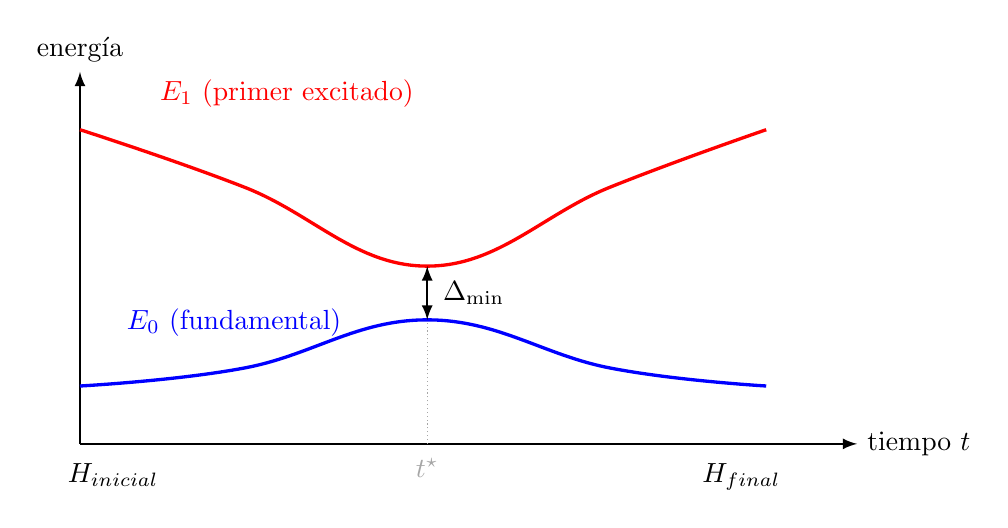
\begin{tikzpicture}[scale=1.05]
    % ejes
    \draw[-latex,thick] (0,0) -- (9.4,0) node[right] {tiempo $t$};
    \draw[-latex,thick] (0,0) -- (0,4.5) node[above] {energía};
    % linea vertical en el instante del gap minimo y region sombreada
    \draw[densely dotted,gray!70] (4.2,0) -- (4.2,2.15);
    \node[gray!70,anchor=north] at (4.2,-0.06) {$t^{\star}$};
    % curva del estado fundamental E0
    \draw[very thick,blue] plot[smooth,tension=0.7]
      coordinates {(0,0.7)(2,0.92)(4.2,1.5)(6.4,0.92)(8.3,0.7)};
    % curva del primer estado excitado E1
    \draw[very thick,red] plot[smooth,tension=0.7]
      coordinates {(0,3.8)(2,3.1)(4.2,2.15)(6.4,3.1)(8.3,3.8)};
    % gap minimo, claramente acotado
    \draw[latex-latex,thick] (4.2,1.5) -- (4.2,2.15) node[midway,right=2pt] {$\Delta_{\min}$};
    % etiquetas de las curvas, en bandas despejadas para no solapar las curvas
    \node[blue,anchor=south west] at (0.45,1.18) {$E_0$ (fundamental)};
    \node[red,anchor=south west] at (0.85,3.95) {$E_1$ (primer excitado)};
    % hamiltonianos inicial y final
    \node[anchor=north] at (0.4,-0.12) {$H_{\text{inicial}}$};
    \node[anchor=north] at (8.0,-0.12) {$H_{\text{final}}$};
  \end{tikzpicture}
  \caption[Esquema de la evolución adiabática]{Esquema de la evolución
    adiabática. El sistema parte del
    estado fundamental de un hamiltoniano sencillo $H_{\text{inicial}}$ y
    se deforma lentamente hacia $H_{\text{final}}$, cuyo fundamental
    codifica la solución. La separación entre el nivel fundamental $E_0$ y
    el primer excitado $E_1$ alcanza un mínimo $\Delta_{\min}$; el teorema
    adiabático exige una evolución lenta frente a ese gap para no abandonar
    el estado fundamental.}
  \label{fig:adiabatica-esquema}
\end{figure}

El factor que gobierna esa exigencia es el gap mínimo $\Delta_{\min}$: la
condición adiabática pide un tiempo de evolución que crece, a grandes
rasgos, como $1/\Delta_{\min}^2$, de modo que las instancias con un gap
pequeño son las más difíciles de resolver sin abandonar el estado
fundamental. Por eso la calidad de la solución depende del diseño de los
\emph{drivings}: los perfiles temporales de los campos de control que
gobiernan la evolución. En el protocolo concreto que emplea el método
evaluado, esos campos son tres: la frecuencia de Rabi $\Omega(t)$, que
mide la intensidad con que el láser acopla los estados $|0\rangle$ y
$|1\rangle$ y, por tanto, la rapidez con que un átomo puede pasar de uno a
otro; el \textit{detuning} global $\Delta(t)$, el desfase entre la
frecuencia del láser de control y la de la transición atómica, que regula
cuántas excitaciones resultan energéticamente favorables; y un
\textit{detuning} local por átomo que codifica la relevancia de cada
variable. Los tres se programan en dos pasos para mantener la
adiabaticidad con tiempos finitos, un problema de control activo en la
literatura~\cite{ding2021, arribas2025}. Al final de
la evolución, la medición del sistema en la base computacional produce
cadenas binarias; repetir el proceso genera una distribución de
soluciones candidatas en la que las configuraciones de menor energía
aparecen con mayor probabilidad.

\section{Átomos neutros y bloqueo de Rydberg}
\label{sec:mt-rydberg}

Las plataformas de átomos neutros confinan átomos individuales
mediante pinzas ópticas, lo que permite disponerlos en geometrías
bidimensionales arbitrarias y reconfigurables~\cite{henriet2020}. Cada
átomo actúa como un cúbit: el estado fundamental representa el valor
0 y un estado de Rydberg altamente excitado representa el valor 1.
Dos átomos excitados simultáneamente a estados de Rydberg
interactúan con una intensidad que decae con la sexta potencia de la
distancia que los separa. Esta interacción, de tipo van der Waals, se
describe como
\begin{equation}
  \label{eq:vdw}
  V_{ij} = \frac{C_6}{r_{ij}^{6}},
\end{equation}
donde $r_{ij}$ es la distancia entre los átomos $i$ y $j$ y $C_6$ un
coeficiente que depende del estado de Rydberg empleado. La fuerte
dependencia con $r_{ij}^{-6}$ es la que hace que la interacción pase de
despreciable a dominante en un margen estrecho de distancias.

De esa interacción surge el fenómeno que explota este trabajo: el
\emph{bloqueo de Rydberg}. Cuando dos átomos están más cerca que una
distancia crítica, llamada radio de bloqueo, la interacción desplaza
tanto la energía del estado doblemente excitado que el láser de
control no puede poblarlo: dentro de un volumen de bloqueo solo cabe
una excitación. El hardware implementa así, de forma nativa, una
restricción dura de exclusión entre vecinos, que es exactamente la
restricción de independencia del MWIS (Figura~\ref{fig:rydberg-esquema}).
Esta correspondencia ha
permitido resolver experimentalmente instancias del conjunto
independiente máximo con cientos de átomos~\cite{ebadi2022} y es la
base del método de selección de características evaluado en este
trabajo~\cite{orquin2026}.

\begin{figure}[!htbp]
  \centering
  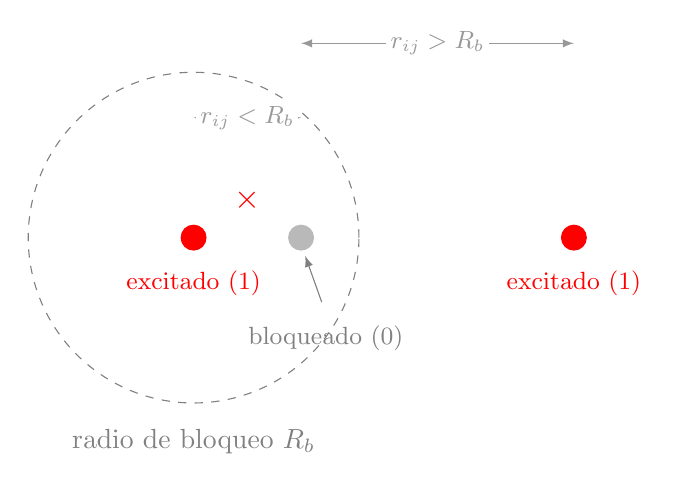
\begin{tikzpicture}[scale=1.05]
    % radio de bloqueo alrededor del atomo excitado izquierdo
    \draw[dashed,gray] (0,0) circle (2.0);
    \node[gray,anchor=north] at (0,-2.2) {radio de bloqueo $R_b$};
    % distancias, arriba y con fondo blanco para no solaparse con nada
    \draw[latex-latex,gray!80] (0,1.45) -- (1.3,1.45)
      node[midway,fill=white,inner sep=1.5pt] {\small $r_{ij}<R_b$};
    \draw[latex-latex,gray!80] (1.3,2.35) -- (4.6,2.35)
      node[midway,fill=white,inner sep=1.5pt] {\small $r_{ij}>R_b$};
    % atomo excitado (1) izquierdo, etiqueta debajo
    \filldraw[red] (0,0) circle (0.15);
    \node[red,anchor=north] at (0,-0.28) {\small excitado ($1$)};
    % atomo vecino dentro del radio -> bloqueado, etiqueta debajo y separada
    \filldraw[gray!55] (1.3,0) circle (0.15);
    \node[gray,anchor=north] at (1.6,-0.95) {\small bloqueado ($0$)};
    \draw[gray,-latex] (1.55,-0.78) -- (1.35,-0.22);
    % cruz de prohibicion entre los dos vecinos
    \node[red] at (0.65,0.45) {\large$\times$};
    % atomo lejano fuera del radio -> puede excitarse
    \filldraw[red] (4.6,0) circle (0.15);
    \node[red,anchor=north] at (4.6,-0.28) {\small excitado ($1$)};
  \end{tikzpicture}
  \caption[Bloqueo de Rydberg]{Bloqueo de Rydberg. Dos átomos dentro
    del radio de bloqueo
    $R_b$ no pueden excitarse a la vez: si uno ocupa el estado de Rydberg
    ($1$), el desplazamiento de energía de van der Waals
    (ecuación~\ref{eq:vdw}) impide poblar el de su vecino, que queda en el
    estado fundamental ($0$). Un átomo fuera de $R_b$ sí puede excitarse.
    Esta exclusión entre vecinos reproduce la restricción de
    independencia del MWIS sobre el grafo de características.}
  \label{fig:rydberg-esquema}
\end{figure}

\section{Herramientas de validación estadística}
\label{sec:mt-validacion}

Un estudio que examina muchas variables con muchos contrastes genera
asociaciones aparentes por puro azar: a un nivel de significación
fijo, la proporción esperada de falsos positivos crece con el número
de contrastes realizados. Este trabajo adopta cuatro salvaguardas
sistemáticas frente a ese riesgo, que se aplican en todas las fases
del bloque experimental: la corrección por multiplicidad sobre la
asociación variable--target, la comprobación de que el preprocesado y
el particionado no alteran el problema, y una cadena de contrastes que
autoriza el diagnóstico final.

Los contrastes empleados son no paramétricos para no depender de la
normalidad. La asociación de una variable numérica con un target de dos
grupos se contrasta con la prueba de rangos de Mann--Whitney~\cite{mann1947},
y con la de Kruskal--Wallis~\cite{kruskal1952} cuando el target tiene
más de dos clases; la asociación entre variables categóricas se contrasta
con la prueba $\chi^2$ de independencia. La monotonía entre dos
ordenaciones (por ejemplo, el ranking de relevancia antes y después del
preprocesado) se mide con la correlación de rangos de Spearman
$\rho\in[-1,1]$, que vale $1$ cuando ambas ordenaciones coinciden. Para
comparar la distribución de una misma variable entre dos particiones se
emplean tres medidas complementarias, todas nulas cuando las
distribuciones coinciden: el estadístico de Kolmogorov--Smirnov, que toma
la máxima distancia vertical entre las funciones de distribución
acumuladas y es sensible a desplazamientos locales; la distancia de
Wasserstein estandarizada, que cuantifica el «coste» de transformar una
distribución en la otra y capta diferencias globales de forma; y el
índice de estabilidad poblacional (PSI), un indicador de uso habitual en
la industria para detectar cambios de población entre dos muestras. El
desplazamiento de la proporción de clases del target entre particiones se
contrasta, además, con la prueba $\chi^2$ y, cuando las frecuencias son
pequeñas, con la prueba exacta de Fisher.

La primera es la corrección por comparaciones múltiples. Cuando se
contrasta una batería de variables contra el target, los p-valores se
ajustan con el procedimiento de Benjamini--Hochberg~\cite{benjamini1995}:
se ordenan los $m$ p-valores de menor a mayor y se rechaza la hipótesis
nula para el mayor $p_{(i)}$ que cumple $p_{(i)} \le \frac{i}{m}\,q$,
con lo que se controla en $q$ la proporción esperada de falsos
descubrimientos (FDR, \textit{False Discovery Rate}). Una variable solo
se considera asociada al target si su contraste sobrevive a esa
corrección, no si resulta significativa de forma aislada.

La segunda es la distinción entre significancia y magnitud. Un
p-valor responde si un resultado es compatible con el azar, no si es
relevante: con tamaños muestrales grandes, efectos minúsculos resultan
estadísticamente significativos. Por ello, cada contraste se acompaña de su tamaño de efecto, acotado y
comparable entre problemas: la delta de Cliff~\cite{cliff1993} para los
contrastes de dos grupos de Mann--Whitney~\cite{mann1947}, que mide en
$[-1,1]$ cuánto tiende un grupo a superar al otro; el épsilon cuadrado
para los de Kruskal--Wallis~\cite{kruskal1952}, que expresa en $[0,1]$
la fracción de variabilidad por rangos atribuible al grupo; y la V de
Cramér para los contrastes de independencia entre variables
categóricas, también en $[0,1]$. La lectura conjunta de significancia y
magnitud es la que sostiene las conclusiones.

La tercera es la construcción de distribuciones nulas empíricas por
permutación. Cuando la distribución nula de un estadístico no es
conocida, como ocurre con las puntuaciones de los selectores de
características, se genera empíricamente permutando el target y
recalculando la puntuación; un valor observado solo se considera señal
si supera el percentil alto de esa distribución nula. El mismo
principio se aplica al rendimiento de los modelos finales mediante la
permutación de etiquetas, que verifica que ningún resultado es
compatible con un clasificador aleatorio.

La cuarta es la cuantificación de la incertidumbre por remuestreo. Los
intervalos de confianza de las métricas de prueba se obtienen por
\textit{bootstrap}~\cite{efron1979} sobre las predicciones, sin
supuestos distribucionales, y las comparaciones entre configuraciones
se realizan de forma pareada sobre las mismas filas. Esta lógica de
contrastar lo observado frente a lo que el azar o el criterio regalan
se extiende a la fase cuántica: la comparación con el óptimo exacto de
la función de coste, descrita en el capítulo de métodos, permite
distinguir la calidad de la optimización de la calidad del criterio
optimizado.

% Estado del arte integrado como sección del marco teórico (antes era el
% Capítulo 3, demasiado corto como capítulo independiente).
\section{Estado del arte}
\label{sec:mt-estado-arte}

Esta sección revisa los trabajos previos sobre los que se apoya la
propuesta, organizados por familias de enfoques. Se examinan primero
los métodos clásicos de selección de características y, a continuación,
las líneas de optimización cuántica de problemas combinatorios y el uso
de átomos de Rydberg en tareas de optimización. La última subsección se
centra en las formulaciones cuánticas de la selección de
características, que constituyen el antecedente directo del método
estudiado.

\subsection{Métodos clásicos de selección de características}

Sobre las tres familias descritas en el marco teórico
(sección~\ref{sec:mt-fs}), la literatura ha consolidado un repertorio de
selectores que reaparecen de forma
recurrente como referencia. Entre los \emph{filter}, la puntuación F de ANOVA
y la información mutua son los criterios supervisados más utilizados por
su bajo coste, y la varianza se mantiene como criterio no supervisado de
control~\cite{solorio2020}. Entre los métodos \emph{embedded}, los más
extendidos son la regularización $\ell_1$ y las importancias por
impureza de los bosques aleatorios~\cite{breiman2001}, mientras que el
criterio mRMR~\cite{peng2005} sigue siendo la referencia para incorporar
la redundancia de forma explícita. Entre los \emph{wrapper}, el algoritmo
Boruta~\cite{kursa2010}, que compara la importancia de cada variable con
la de copias permutadas (variables \textit{sombra}) y retiene solo las
que la superan de forma consistente, se ha convertido en uno de los
puntos de comparación habituales en la literatura reciente de selección
cuántica, pese a que su coste crece con los reentrenos del modelo base.

Esa misma literatura ha señalado que el rendimiento predictivo no basta
para caracterizar un selector. La estabilidad de los subconjuntos ante
perturbaciones como el cambio de semilla o de muestra se cuantifica con
índices de solape corregidos por azar, como el de
Kuncheva~\cite{kuncheva2007}: un selector inestable produce subconjuntos
poco reproducibles aunque su rendimiento medio sea alto. La estabilidad
y la redundancia interna se han establecido así como dimensiones de
evaluación complementarias al rendimiento.

\subsection{Optimización cuántica de problemas combinatorios}

La resolución de problemas QUBO es una de las aplicaciones más
estudiadas de la computación cuántica actual~\cite{schuld2021,
wittek2014}. Se han explorado tres líneas principales: el
\textit{quantum annealing} o recocido cuántico, un hardware dedicado que
relaja lentamente el sistema hacia el estado fundamental de un
hamiltoniano para hallar el mínimo de la función de coste; los algoritmos
variacionales sobre procesadores de puertas; y la simulación
hamiltoniana analógica sobre plataformas como los átomos neutros. Las
tres comparten el mismo esquema conceptual, codificar la función de
coste en un hamiltoniano y buscar su estado fundamental, y se
diferencian en el mecanismo de búsqueda y en las restricciones que el
hardware impone al problema. Para problemas con restricciones de
exclusión, la vía analógica resulta especialmente natural porque la
propia física implementa la restricción, sin penalizaciones añadidas
en la función de coste.

\subsection{Átomos de Rydberg en optimización}

La demostración experimental de mayor escala de esta vía es la
resolución del conjunto independiente máximo sobre grafos de discos
unitarios con matrices de hasta 289 átomos~\cite{ebadi2022}, que
mostró tanto el potencial de la plataforma como la dependencia del
rendimiento respecto de la dureza de la instancia. En paralelo, una
línea activa de investigación, a la que pertenece el grupo en el que
se enmarca este TFG, estudia cómo diseñar los perfiles de control
para preservar la adiabaticidad: desde el control asistido por
aprendizaje profundo~\cite{ding2021} hasta la optimización de
\textit{drivings} y la caracterización espectral de la dificultad de
instancias MWIS en simuladores de átomos neutros~\cite{arribas2025}.
Estos trabajos delimitan qué tamaños y geometrías de problema son
tratables hoy en simulación y motivan la envolvente operativa que se
define en el capítulo~\ref{cap:metodos}.

\subsection{Selección de características mediante formulaciones cuánticas}

La formulación de la selección de características como problema QUBO,
combinando relevancia e información mutua par a par, fue introducida
por Mücke et al.~\cite{mucke2023}, que la evaluaron sobre hardware
cuántico de puertas y \textit{annealers} con resultados competitivos
frente a heurísticas clásicas en problemas de tamaño moderado. Sobre
átomos neutros, la propuesta de referencia es el método QFS del grupo
en el que se desarrolla este trabajo~\cite{orquin2026}, que adapta esa
misma formulación QUBO al hardware de Rydberg: codifica la relevancia
por información mutua en los campos de control locales y la redundancia
en la disposición espacial de los átomos. En sus experimentos sobre
problemas binarios de hasta una veintena de variables, QFS iguala el
área bajo la curva de Boruta empleando subconjuntos más compactos y, en
uno de los conjuntos, la supera. Un hallazgo relevante de esa
evaluación es que el rendimiento se estabiliza más allá de unas siete
variables, lo que sugiere que Boruta tiende a sobreestimar el número de
características relevantes; el método cuántico ofrece subconjuntos más
parcos sin pérdida apreciable. La propia línea de trabajo contrasta
además las soluciones del simulador con el óptimo de la formulación
QUBO obtenido mediante optimización clásica exacta~\cite{orquin2026},
una práctica de control que la evaluación diseñada en este trabajo
adopta.

El hueco que este TFG aborda se sitúa precisamente ahí: la evidencia
preliminar disponible del método se limita a problemas binarios de
dimensionalidad moderada, evaluados con un único protocolo de
clasificación. Queda pendiente una evaluación contra una referencia
clásica contrastada que cubra también escenarios multiclase,
desbalanceados y de alta dimensionalidad.

La laguna no es únicamente cuantitativa. Para valorar un método como
QFS no basta con registrar si iguala o no al baseline: su función de
coste mezcla relevancia y redundancia, y su implementación física añade
un segundo nivel de dificultad al embebido geométrico y a la dinámica
analógica. Por ello, una evaluación útil debe permitir separar tres
preguntas: qué régimen del dato se está resolviendo, qué familia de
selectores clásicos constituye el espejo apropiado y si un fallo, en
caso de aparecer, procede del criterio o del optimizador. Construir esa
referencia y convertirla en un diagnóstico variable a variable es la
contribución de este trabajo.


\section{Integración del marco teórico en el TFG}
\label{sec:mt-integracion}

Las piezas anteriores forman una única cadena, que el
capítulo~\ref{cap:metodos} concreta en un método operativo. La
selección con compromiso relevancia--redundancia
(sección~\ref{sec:mt-fs}) se formula como un QUBO que se aproxima por
un grafo MWIS físico (sección~\ref{sec:mt-qubo}); ese grafo se
materializa en una matriz de átomos neutros, donde la relevancia se
codifica en los \textit{detunings} locales y la redundancia en las
distancias, de modo que el bloqueo de Rydberg
(sección~\ref{sec:mt-rydberg}) impone exclusiones entre variables
redundantes; y una evolución adiabática
(sección~\ref{sec:mt-adiabatica}) lleva el sistema al mínimo de energía,
cuya medición devuelve los subconjuntos candidatos.
